\documentclass{article}
\usepackage[margin=0.8in]{geometry} % change this parameter to enlarge/restrict the margins
\usepackage{amsmath,amsthm,amssymb,amsfonts, fancyhdr, color, comment, graphicx, environ}
\usepackage{xcolor}
\usepackage{mdframed}
\usepackage[shortlabels]{enumitem}
\usepackage{hyperref}
\usepackage{calrsfs}
\DeclareMathAlphabet{\pazocal}{OMS}{zplm}{m}{n}
\usepackage{graphicx}
\usepackage{makecell} %table cells
\usepackage{booktabs} %table appearance
\usepackage{caption} %table caption

\renewcommand{\footrulewidth}{0.8pt}
\hypersetup{
	colorlinks=true,
	linkcolor=blue,
	filecolor=magenta,      
	urlcolor=blue,
}

%/ Margin
%/ ##########################
%/\addtolength{\oddsidemargin}{-.7in}
%/\addtolength{\evensidemargin}{-.7in}
%/\addtolength{\textwidth}{1.4in} %/Double of the 2 above
% ###########################

% fancy style 
\pagestyle{fancy}
% remove fancy style from bottom 
\renewcommand{\footrulewidth}{0pt}

\lhead{Group 20}
\rhead{Algorithmic Machine Learning} 

\newcommand{\loss}{L(\theta, a)}
\newcommand{\lossRule}{L(\theta, \delta(x))}
\newcommand{\risk}{R(\theta, \delta)}

%------------------------------------------------
%% Bibliography
%\usepackage[sorting=none, backend=bibtex]{biblatex}
%\addbibresource{ref.bib}
%------------------------------------------------

\begin{document}
	\title{\Large Algorithmic Machine Learning  \\[0.5cm]
	\bf\Large Challenge 1 - Report \\[0.5cm]
	
	\bf\Large Group 20}

\author{\large 
	\begin{tabular}{rl}
		\textbf{Professor:} & Pietro Michiardi \\
		\textbf{Authors:} & Daniele Falcetta \\ & Simone Papicchio \\ & Massimiliano Pronesti \\ & Federico Tiblias
	\end{tabular}
	}
\date{\large \today}

\makeatletter
\begin{titlepage}
	\begin{center}
		{ 
\includegraphics[width=10cm]{assets/eurecom.png}}
		{\ \\ \ \\}
		\vbox{}\vspace{5cm}
		{\@title }\\[3cm]
		{\@author}\\[3cm]
		{\@date\\}
		
	\end{center}
\end{titlepage}
\makeatother
	
\section{Introduction}
    The Weather Forecast problem consists in using pairs of meteorological features and target values at a particular latitude/longitude and time to predict the air temperature measurements at 2 meters above the ground. The dataset contains 112 features which are either direct measurements (such as sun elevation at the current location, humidity, temperature, pressure and topography, and other meteorological parameters) or weather predictions provided by climatic models (Global Forecast System, Global Deterministic Forecast System from the Canadian Meteorological Center, Weather Research and Forecasting). Each model returns the following predicted values: wind, humidity, pressure, clouds, precipitation, dew point, snow depth, air and soil temperature characteristics. Where applicable, the predictions are given at different isobaric levels from 50 hPa (20 km above ground) to the ground level. The features are highly heterogeneous, i.e. they are of different types and scales and are highly correlated between each other. Most importantly, this dataset is afflicted by a serious shift between train and test distributions. 
    
    Dataset shifting is a phenomenon that occurs when the distribution of the train and test data differs. This may cause several problems because the model is trained on one distribution but is used to make predictions on a different one, resulting in poor results. There are different types of data shifting such as 
    Covariance Shift\footnote{Changes in the independent variables or features of the dataset},
    Probability Shift\footnote{Changes in the target variable or the dependent variable in the dataset}
    and Concept Shift.\footnote{Change in the connection between the independent and the target variable across datasets}
    In this work we analyze the presence of the Spatial Covariance Shift and try to address its main challenges. A visualization of the difference in distribution for the datapoints can be seen in Fig. \ref{fig:train-test-diff}.
    

    \begin{figure}[h]
        \centering
        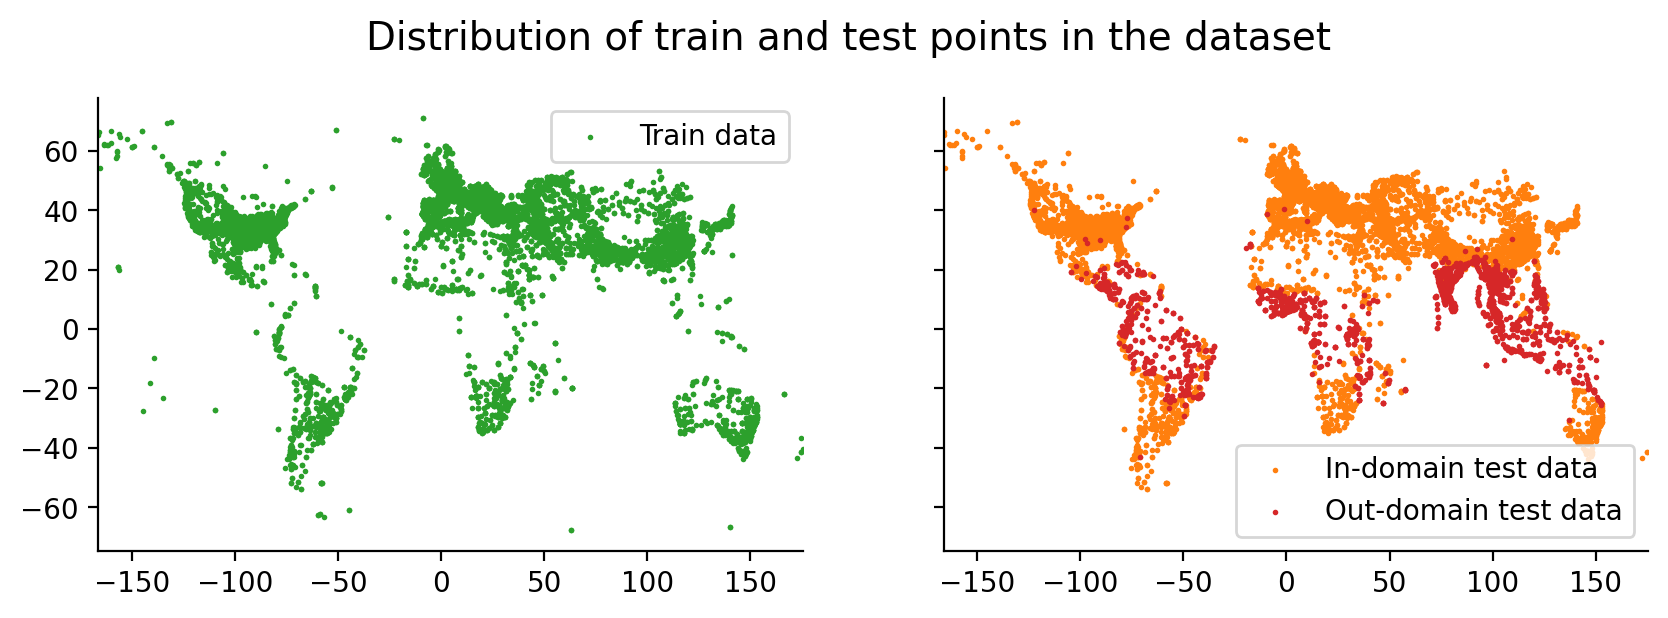
\includegraphics[width=\linewidth]{assets/train-test-diff.png}
        \caption{The figure clearly shows that the regions in the range of latitude from -18 to 10 are not present in the train dataset. This phenomenon is called \textit{Spatial Covariance Shift}.}
        \label{fig:train-test-diff}
    \end{figure}

\section{Data Analysis}
    \subsection{Outliers}
    The first step of our dataset analysis focuses on outliers detection. Our approach, based on the Interquartile method (IQR), consists in plotting a boxplot for each feature. To obtain better and more organized visualizations, we plot four different graphs, one for each weather forecast model and, given the high heterogeneity of the features, we scale our data between 0 and 1 according to a min-max normalization. This analysis shows that almost all the features contain some outliers. In Section 3 we show some experiments attempting to remove part or all of them. A particular mention has to be done for the feature \textit{gfs\_soil\_temperature}, which contains some entries equal to -9999 °C, i.e. a missing measurement, as reported in the associated feature \textit{gfs\_soil\_temperature\_available}.
    
    \subsection{Correlations}
    Understanding the correlations among the features in the dataset is another crucial point since it can affect the results of some models. We start analyzing the correlation between the features and the target. Table \ref{table:pearsCorr} shows the ten features that correlate most with the target. An approximate analysis would lead to the removal of all the other features. However, this approach might be inaccurate: the Pearson coefficient only analyzes linear correlations, without taking into account non linear ones. In addition, we are not bearing into consideration that features might correlate between each other. If this is the case, two highly correlated features carry the very same information and one of them can be dropped. Conducting this analysis, we figured that the \textit{gfs\_temperature\_xxxxx} features are in fact correlated when they are in similar conditions\footnote{The temperature measurements are taken in close isobaric levels}. The same kind of correlation can be detected among other groups of features.  

    \subsection{Feature Shift}
    Train and test datasets show a noticeable shift in the distribution of samples: test datapoints are distributed homogeneously around the globe, while the train dataset lacks samples in the equatorial region. To gain a deeper understanding of how this phenomenon affects our prediction, we compute a metric reminiscent of the Wasserstein distance. For each feature we divide the dataset into 100 bins of equal size and normalize them in order to obtain histograms. Then, we compute the area difference between the cumulative sum of these histograms for train and test datasets. The value we obtain represents some notion of distance between the two distributions and can be used later on during feature selection. Table \ref{table:wassDist} reports the ten most shifted features according to this metric. 

\vspace{0.5cm}    
\setlength{\tabcolsep}{8pt}
\hspace{-0.5cm}\begin{minipage}[c]{0.5\textwidth}
\centering
\begin{tabular}{lccl}
\toprule
\makecell{Feature}                         & \makecell[t]{Pearson\\ Correlation} \\ \midrule
\textbf{wrf\_t2\_interpolated}   & \textbf{0.963}     \\
wrf\_t2\_next                   & 0.958               \\
gfs\_temperature\_97500         & 0.874               \\
gfs\_temperature\_95000         & 0.863               \\
climate\_temperature            & 0.857               \\
gfs\_temperature\_92500         & 0.852               \\
gfs\_temperature\_90000         & 0.842               \\
gfs\_temperature\_85000         & 0.824               \\
gfs\_temperature\_80000         & 0.808               \\
cmc\_0\_0\_6\_2                 & 0.807               \\ \bottomrule

\end{tabular}
\captionsetup{width=0.8\linewidth}
\captionof{table}{Features most correlated to target value in the training dataset according to Pearson metric.}
\label{table:pearsCorr}
\end{minipage}
\begin{minipage}[r]{0.5\textwidth}
\centering
\begin{tabular}{lccl}
\toprule
\makecell[c]{Feature}                         & \makecell[t]{Wasserstein\\ distance} \\ \midrule
\textbf{wrf\_available}                  & \textbf{49.000 }\\
\textbf{gfs\_available}                  & \textbf{49.000 }\\
\textbf{cmc\_available}                  & \textbf{49.000 }\\
gfs\_2m\_dewpoint\_grad         & 24.006               \\
cmc\_0\_1\_0\_0                 & 17.057               \\
gfs\_precipitable\_water        & 16.999               \\
gfs\_v\_wind                    & 16.866               \\
gfs\_temperature\_15000         & 14.541               \\
gfs\_total\_clouds\_cover\_high & 13.718               \\
fact\_latitude                  & 13.625               \\
\bottomrule
\end{tabular}
\captionsetup{width=0.8\linewidth}
\captionof{table}{Most shifted features between train and test datasets according to Wasserstein metric.}
\label{table:wassDist}
\end{minipage}

%\begin{table}
%\begin{center}
%\begin{tabular}{lccl}
%\toprule
%Feature                         & Wasserstein distance \\ \midrule
%fact\_latitude                  & 13.625               \\
%gfs\_total\_clouds\_cover\_high & 13.718               \\
%gfs\_temperature\_15000         & 14.541               \\
%gfs\_v\_wind                    & 16.866               \\
%gfs\_precipitable\_water        & 16.999               \\
%cmc\_0\_1\_0\_0                 & 17.057               \\
%gfs\_2m\_dewpoint\_grad         & 24.006               \\
%cmc\_available                  & 49.000               \\
%gfs\_available                  & 49.000               \\
%wrf\_available                  & 49.000               \\ \bottomrule
%\end{tabular}
%\end{center}
%\captionof{table}{Most shifted features between train and test dataset according to Wasserstein metric.} 
%\end{table}


\section{Pre-Processing}
Different models call for different preprocessings and feature selections. We try different approaches in conjunction with one or more models to find the best one in each situation.
\begin{itemize}
    \item \textbf{Dealing with missing values:} either fill missing values with their respective column mean or drop samples containing at least one NaN.
    \item \textbf{Outlier removal:} either remove all datapoints outside of the interquartile range or use sklearn's \textit{LocalOutlierFactor} to detect and exclude outliers.
    \item \textbf{Rescaling:} normalize all features using sklearn's \textit{StandardScaler}.
    \item \textbf{Feature selection based on Random Forest feature importance:} to address the correlation issues mentioned earlier, we keep only the 20 most important features according to a Random Forest Regressor\footnote{\textit{n\_estimators}=10, \textit{max\_depth}=30}. Interestingly, the first four features represent almost the totality of importance (Tab. \ref{table:featImpo}).
    
    \item \textbf{Feature selection based on Wasserstein distance:} rank features according to the metric described in Subsection 2.3 and keep only the $n$ less-shifted ones as they should better represent the test distribution.
    \item \textbf{PCA:} correlation analysis shows many features are correlated, this poses a problem for linear models. We address this issue by performing a PCA keeping either \textit{num\_features} - 1 principal components or by selecting the components explaining $99\%$ of variance.
    \item \textbf{Daylight and hour:} use \textit{fact\_time, fact\_latitude, fact\_longitude} to compute the hour of day and the amount of daylight received in the day the measurement took place.
\end{itemize}
\begin{center}
\begin{tabular}{cc}
\toprule
\makecell{Feature}& \makecell[t]{Importances} \\
\midrule
\textbf{wrf\_t2\_interpolated}     & \textbf{0.871038}\\
gfs\_temperature\_97500   & 0.034633\\
cmc\_0\_0\_6\_2             & 0.011729\\
climate\_temperature     & 0.010516\\
wrf\_snow                & 0.004567\\
sun\_elevation           & 0.004368 \\
cmc\_0\_0\_7\_2             & 0.004134\\
cmc\_0\_1\_0\_0             & 0.003386\\
gfs\_soil\_temperature    & 0.002967\\
fact\_longitude          & 0.002202\\
\bottomrule
\end{tabular}
\captionsetup{width=0.8\linewidth}
\captionof{table}{The 10 most important features extracted with a Random Forest with 10 trees and max depth equal to 30}
\label{table:featImpo}
\end{center}


    \section{Models}
    We perform an initial exploratory analysis comparing a variety of models along with different preprocessings and pick the ones that perform best to be further explored with hyper-parameter tuning. 
    
    We start our analysis with a simple explainable model, \textbf{Ridge}. The main challenge in its usage is to remove the collinearity present in the dataset. To do this we use techniques such as Principal Component Analysis and feature selection with a Random Forest. 
    
    Since it is possible that the relationship between target and features is non-linear, we move to a \textbf{Random Forest Regressor}. It proves very effective even for a small number of estimators. However, the training time of the model rapidly increases with forest size.
    
    In order to get even better, we move to boosting techniques. Among the several models available, we use \textbf{CatBoost} which is a decision tree boosting algorithm. CatBoost builds a set of decision trees consecutively, each one with reduced loss compared to the previous ones. This procedure is repeated for the specified number of iterations.

    \section{Hyper-parameter tuning}
    We perform for each model a simple Grid Search on a small amount of hyperparameters with a five-fold cross validation. By comparing the train and validation scores on the best split we select the best performing model and its respective best set of hyperparameters.

    To avoid data leakage between train and validation sets we pack both preprocessing and model in a Pipeline\footnote{sklearn.pipeline.Pipeline} that is repeated on each iteration of the five-fold.
    
\setlength{\tabcolsep}{1.9em}
\begin{table*}[t]
\centering
\begin{tabular}{p{2cm}p{4.5cm}p{1.8cm}p{2cm}}
\toprule

\makecell[t]{Pipeline \\ \& Model} & \makecell[t]{Hyperparameters \\ Explored} & \makecell[t]{Best} & \makecell[t]{Validation \\ RMSE}\\
\midrule
% first row
\makecell{StandardScaler,\\ PCA, \\ Ridge}  & \makecell{ \\ alpha: [0.1, 0.01, 0.001]} & \makecell{\\ alpha: 0.1} & \makecell[t]{\\2.4}\\
%second row
\makecell{StandardScaler, \\ 20 RF features \\ Ridge} & \makecell{\\alpha: [0.1, 0.01, 0.001]} & \makecell{ \\ alpha: 0.1} & \makecell{\\2.71}\\
%third row
\makecell{StandardScaler, \\ 20 RF features\\ Random Forest } & \makecell{ \\ \\ n\_estimators: [2, 5, 8, 10]\\max\_depth: [15, 30, 60]} & \makecell{ n\_estimators: 10\\max\_depth: 30} & \makecell{\\2.76}\\
%fourth row
\makecell{\textbf{StandardScaler,}\\ \textbf{CatBoostReg}} & \makecell{\\ \\ lr: [0.1, 0.01], depth:[8,10]\\iterations:[1000, 10000]} & \makecell{lr: 0.1, depth: 10 \\iterations:10000} & \makecell{\\1.52}\\
      



\bottomrule
\end{tabular}
\captionof{table}{Models and hyperparameters tested} 
\label{table:hypTest}
\end{table*}
\section{Results}
Applying different combinations of preprocessing techniques, we observe the following outcomes:

\begin{itemize} 
    \item Filling missing values with the column mean or dropping the sample altogether produces comparable results. We choose to always fill with the mean to avoid dropping potentially useful samples;
    \item Regardless of the outliers removal technique we tried over distinct experiments, we obtain our best results by keeping the outliers in the analysis;
    \item Rescaling proves always useful in improving performances;
    \item Despite our efforts in coming up with sensible metrics for feature selection, we find that keeping all features and letting the model choose the most important ones during training is still the best-performing approach also in the presence of spatial shift;
    \item PCA is needed only for linear models to avoid collinearity. This leads to noticeable improvements on the train and test scores at the cost of explainability, as PCA changes the basis in which data is represented. Other models show a reduction in performance when PCA is applied;
    \item Daylight and hour do not lead to any noticeable improvements on any analyzed model. This is possibly due to the feature \textit{sun\_elevation} representing similar informations.
\end{itemize} 

Regarding the models, we obtain increasingly better results as the complexity of the model increases. Indeed, the best performing model is the CatBoost regressor with a validation score of 1.52. Despite the results, dealing with more complex models has many drawbacks such as the loss of explainability or the increasing time complexity.

These results suggest that this dataset hardly requires any preprocessing or feature selection. The highest scoring methods either perform regularization or implicit feature selection thanks to trees, showing that an automatic choice of features wins over a curated manual one. This does not surprise us: plenty of features correlate extremely with the target and require no fancy transformation to be used effectively by the models.

\section{Conclusions}
We show a simple way in which Catboost can be used to predict temperature measurement with very little preprocessing required. This solution yields very good results despite its simplicity.

Despite consisting of almost 2 million measurements, the actual weather stations are few in number, totaling around 5000. A more detailed analysis could investigate aggregates of measurements coming from the same station in order to increase performance. An even more refined approach would be to group together measurements coming from the same station and treat the prediction as a time series problem, applying models such as RNNs and LSTM.

\end{document}